\chapter{Related work}\label{ch:related_work}
From a computer vision perspective, the human body can be considered as a collection of rigid parts or limbs connected by a number of joints~\cite{Gong2016-kd}. Following this approach, the goal of human pose estimation methods is to determine the two-dimensional or three-dimensional location of these joints and parts within an image or a sequence of images. In this chapter, we explore previous work in the field of human pose estimation. We start presenting solutions for 2D pose estimation, categorized as classic approaches and \gls{dl}-based solutions. The former rely on optimizations of explicit human body models to infer poses, while the latter are based on \gls{dl} models with different architectures and training techniques. Then, 3D pose estimation methods are presented and categorized depending on the nature of the input data, \ie RGB or RGBD images.

\section{2D Estimation}\label{sec:2d_estimation}
\subsection{Classic methods}\label{subsec:classic_2d_estimation}
Conventional human pose estimation methods portray the human body as an articulated object. In that sense, most of the early works in the field present part-based models as a solution, not only for estimating human poses, but as tools for modeling any kind of object that can be interpreted as a collection of connected keypoints, \eg hands or faces. Such is the case of the novel pictorial structures model proposed by Fischler and Elschlager~\cite{Fischler1973-bi}. In their work, they model objects as a collection of parts arranged in a deformable configuration, in which pairs of parts are linked by spring-like connections. The model is optimized by minimizing an energy function that measures a match cost for each part and a deformation cost for each of these spring-like links between pairs. In Figure~\ref{subfig:fischler}, we can see the intuitiveness of pictorial structures, exemplified in a diagram that models the human face.

\begin{figure}[h]\centering
    \begin{subfigure}{0.49\textwidth}\centering
        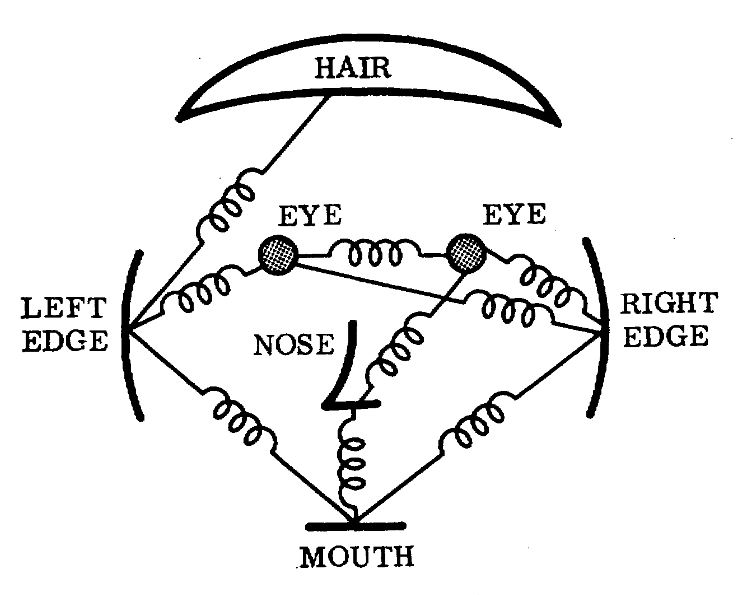
\includegraphics[height=5.75cm]{figures/fischler.jpg} 
        \caption{Human face as a pictorial structure~\cite{Fischler1973-bi}.}
        \label{subfig:fischler}
    \end{subfigure}
    \begin{subfigure}{0.49\textwidth}\centering
        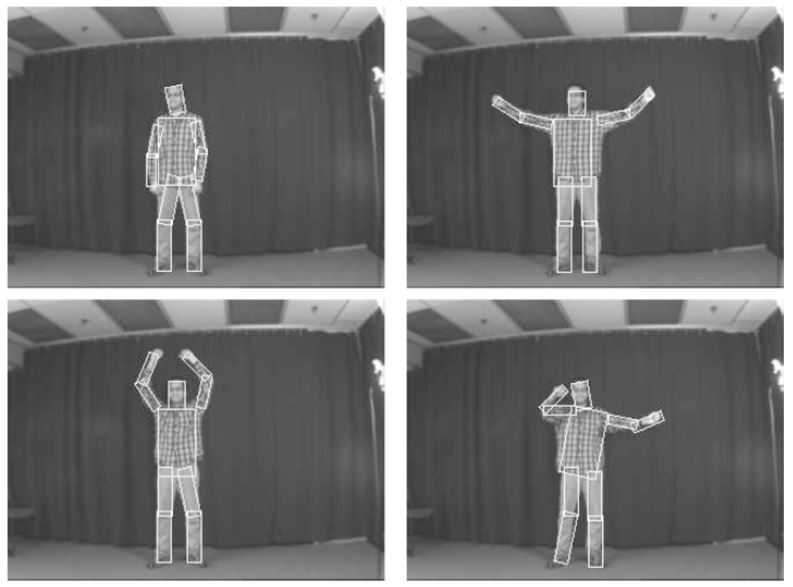
\includegraphics[height=5.75cm]{figures/felzenszwalb.jpg}
        \caption{Pictorial structures application~\cite{felzenszwalb2005pictorial}.}
        \label{subfig:felzenszwalb}
    \end{subfigure}
    \caption{In (a), a human face is modeled as a pictorial structure, as originally introduced by Fischler and Elschlager~\cite{Fischler1973-bi}. In (b), results of applying pictorial structures to the human pose estimation problem, as revisited by Felzenszwalb and Huttenlocher~\cite{felzenszwalb2005pictorial}.}
    \label{fig:pictorial_structures}
\end{figure}

To the best of our knowledge, Felzenszwalb and Huttenlocher~\cite{felzenszwalb2005pictorial} introduced the application of pictorial structures to the recognition of human body poses. Figure~\ref{subfig:felzenszwalb} presents some of their results. The main improvements with respect to the original work are the consideration of models with acyclic connections, which better matches the appearance of human bodies, and the inclusion of a supervised learning algorithm for the optimization stage. Their model also allows the detection of multiple instances of the objects recognized in the images. Other examples of successful extensions of the pictorial structures model for human pose estimation can be found in the works of Andriluka \etal\cite{Andriluka2009-on} and Yang and Ramanan~\cite{Yang2011-vn}. The latter propose a mixture of non-oriented pictorial structures, which further improves the representation of the human body. They use \emph{Histograms of Oriented Gradients} as features and fit the model parameters using \emph{Support Vector Machines}. Their method outperformed previous approaches dramatically in terms of both accuracy and efficiency.

The list of works that propose new appearance models or extensions of the ones mentioned above goes on and on~\cite{Sapp2010-dm, Pishchulin2013-zi, Kiefel2014-vm, Wang2013-wv}. It is worth mentioning the adaptation presented by Eichner and Ferrari, which is able of dealing with multiple subjects in the images. Their model takes into account the spatial relation between multiple human poses and how they occlude each other. Another active field of study is the inclusion of spatio-temporal cues for estimation in video sequences~\cite{Cherian2014-zf, Fathi2007-dc, Ferrari2008-ry, Zhang2015-js}.

\subsection{Deep learning based methods}\label{subsec:dl_2d_estimation}
% presentation of more holistic approaches with the first steps into DNN
More holistic approaches started to gain popularity with the inclusion of \gls{dl} techniques. In~\cite{Toshev2014-ou}, Toshev and Szegedy explore the application of \glspl{cnn} to estimate the body joints locations considering a cascade of \emph{Deep Neural Networks} which refines a coarse initial estimation. In~\cite{Tompson2014-iq}, Tompson \etal propose a joint training of a hybrid architecture composed of a \gls{cnn} (as the part detector) with a part-based spatial model inspired on \emph{Markov Random Fields}, significantly outperforming previous methods. Figure~\ref{fig:tompson} shows how this method is capable of dealing with very complex poses and self-occlusions in images taken \emph{in the wild}.

\begin{figure}[h]
    \centering
    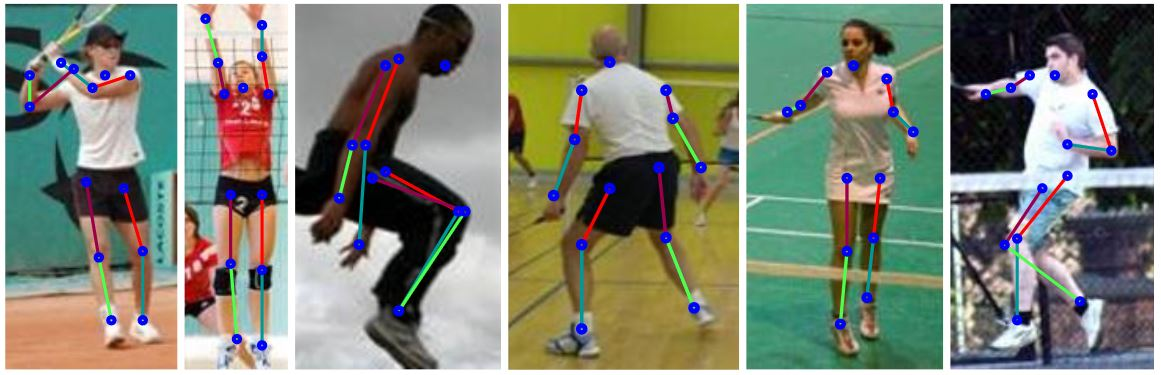
\includegraphics[width=\textwidth]{figures/tompson.JPG}
    \caption{Examples of human poses estimated using the hybrid architecture proposed by Tompson \etal\cite{Tompson2014-iq}.}
    \label{fig:tompson}
\end{figure}

From these works, most research in human pose estimation has shifted towards \gls{dl}-based solutions. Newell \etal\cite{Newell2016-cy} propose a novel \gls{cnn} architecture for this particular task forcing \textit{bottom-up} and \textit{top-down} processing with intermediate supervision. In~\cite{Wei2016-rb}, Wei \etal inherit the \textit{Pose Machines} architecture proposed by Ramakrishna \etal\cite{Ramakrishna2014-ul}, but introducing \glspl{cnn} as feature detectors. Their sequential model, based on multiple stages which take as input belief maps from the previous stages, enables learning long-range dependencies among parts. A more general approach for spatial localization tasks is proposed by Gkioxari \etal\cite{Gkioxari2016-ix}. Because of their intuitiveness and performance, we have chosen these methods (\cite{Newell2016-cy},~\cite{Wei2016-rb} and~\cite{Gkioxari2016-ix}) as 2D human pose estimators for our work. We will further describe their architectures and learning strategies in Chapter~\ref{ch:proposed_method}.

One of the most successful works published in the last years is the one proposed by Chen \etal\cite{Chen2017-pd}. In order to deal with joint occlusions and overlapping of human body parts, they propose the usage of structure-aware \glspl{cnn} and \emph{Generative Adversarial Networks} to train a pose generator only yielding plausible poses, implicitly learning priors about the human body structure. This approach is out of the scope of this paper because, to the best of our knowledge, there is no open source code available.

% 2D estimation with peculiar stuff like multiperson and video
The aforementioned works are focused on 2D pose estimation from individuals on single images. However, several authors have also tried to apply \gls{dl}-based techniques by taking advantage of the temporal information provided by sequences of images~\cite{Jain2015-zb, Pfister2015-ae, Song2017-fe, Girdhar2018-lx}. Such is the case of Pfister \etal\cite{Pfister2015-ae}, who introduce in their pipeline dense optical flow estimations to warp estimated per-joint heatmaps in consecutive frames. In that way, the trained \gls{cnn} is forced to learn the temporal relationships between sequences of poses. Another approach to human pose estimation in 2D video is proposed by Girdhar \etal\cite{Girdhar2018-lx}. In their work, they propose a 3D extension of the \emph{Mask R-\gls{cnn}} architecture~\cite{he2017mask} to couple spatio-temporal information. \gls{dl}-based methods have also been employed in multi-person scenarios~\cite{cao2018openpose, Iqbal2017-nu, Papandreou2017-nk, Insafutdinov2017-zx} and dense pose estimations, which map image pixels of the human body to its corresponding 3D surface~\cite{Alp_Guler2018-rg}. In Figure~\ref{fig:multiperson_and_dense}, examples of multi-person and dense pose estimations are shown.

\begin{figure}[h]\centering
    \begin{subfigure}{0.53\textwidth}\centering
        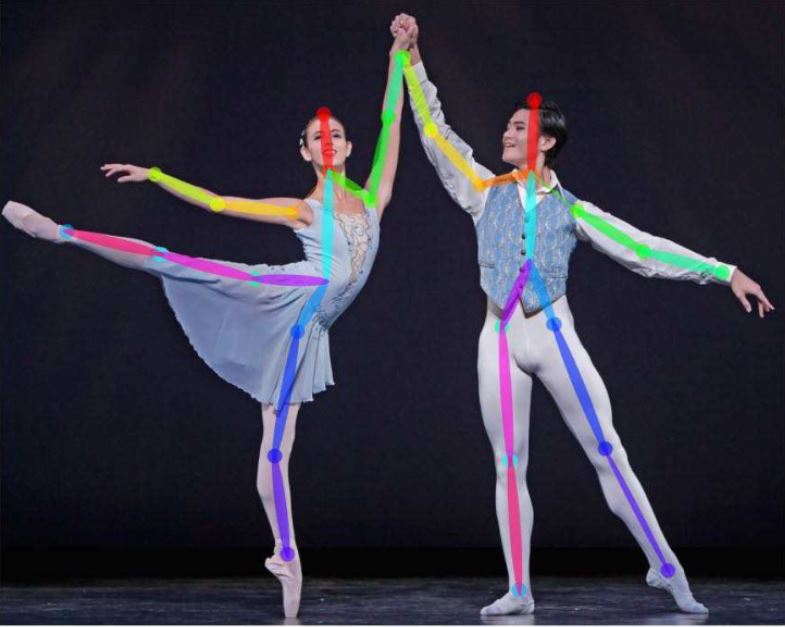
\includegraphics[height=6.5cm]{figures/multiperson.jpg} 
        \caption{Multi-person pose estimation~\cite{cao2018openpose}}
        \label{subfig:multiperson}
    \end{subfigure}
    \begin{subfigure}{0.46\textwidth}\centering
        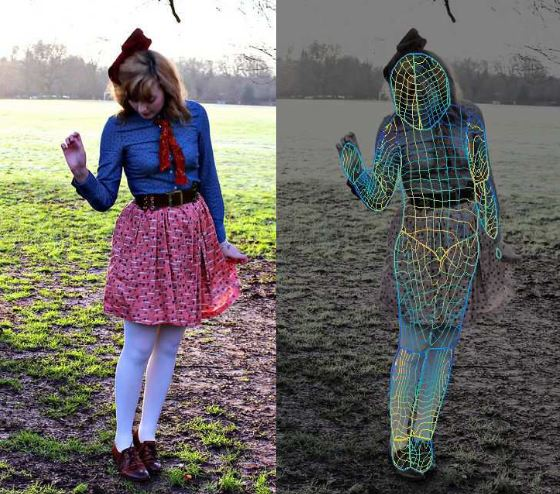
\includegraphics[height=6.5cm]{figures/dense.jpg}
        \caption{Dense pose estimation~\cite{Alp_Guler2018-rg}.}
        \label{subfig:dense}
    \end{subfigure}
    \caption{Besides the more classic scenario of detecting human joints for a single subject, a lot of efforts have been made to tackle down more complex problems. Such is the case of (a) multi-person and (b) dense pose estimations.}
    \label{fig:multiperson_and_dense}
\end{figure}

A major landmark in the field of human pose estimation from RGB images is the development of the \emph{OpenPose} suite~\cite{cao2018openpose}. \emph{OpenPose} is an \emph{open-source} software developed mostly by researchers of the \emph{Carnegie Mellon University}. It builds upon the works in single human pose estimation by Wei \etal\cite{Wei2016-rb}, multi-person pose estimation by Cao \etal\cite{cao2018openpose} and hand pose estimation by Simon \etal\cite{simon2017hand}. They claim the \emph{CMU Panoptic Studio} dataset~\cite{joo2015panoptic} as a core element for their software. Their SDK provides real-time keypoint detection for full human body, hands, feet and face poses.

\section{3D Estimation}\label{subsec:dl_3d_estimation}
\subsection{From RGB images}\label{subsec:from_rgb_images}
Estimating 3D locations from their 2D projections is a highly ill-posed problem, as very different 3D poses can generate very similar 2D projections. However, the \emph{a priori} knowledge about the human body and its plausible poses have allowed researchers to tackle this problem by means of hybrid approaches composed of two-stages: 2D estimation and 3D reconstruction from 2D projections. For instance, Andriluka \etal\cite{Andriluka2010-oc} propose a complete framework for multi-person pose detection in videos using \emph{tracking-by-detection} and 3D exemplars. Regarding the 3D reconstruction from 2D projections, Ramakrishna \etal\cite{Ramakrishna2012-ti} propose an optimization proxy which jointly estimates 3D coordinates from 2D locations of anatomical landmarks and camera parameters while enforcing anthropometric regularity.

Most recent methods introduce \glspl{cnn} for 3D estimation. Chen and Ramanan~\cite{Chen2017-ug} make use of the \glspl{cpm} proposed by Wei \etal\cite{Wei2016-rb} for 2D estimation and then match the resulting pose with a library of 3D exemplars. In~\cite{Bogo2016-kk}, Bogo \etal estimate 2D poses with the \emph{DeepCut} model proposed by Pischulin \etal\cite{Pishchulin2013-zi} and then fit a statistical body shape model to the resulting 2D joints. However, \gls{dl}-based methods have not only been used for the 2D pose estimations, but they have also proved to be a very straight-forward and effective solution for inferring 3D from 2D poses. Thus, Zhou \etal\cite{Zhang2015-js} propose the inclusion of a depth regression module taking the 2D heatmaps generated by a \gls{cnn} as input, providing a 3D pose estimation as the output. A simple but effective approach is proposed by Martinez \etal\cite{Martinez2017-su} by training a \emph{Deep Neural Network} to estimate 3D body joint locations from the corresponding 2D positions. For an adequate performance of the trained model, they consider the inverse transform of the camera to preprocess the 3D ground-truth before training, thus making the 2D to 3D problem similar across different cameras. Tome \etal\cite{Tome2017-ja} propose a more sophisticated solution which not only predicts 3D poses but also uses them to improve their previous 2D estimation, blurring the lines between the two previously mentioned stages.

Several authors~\cite{Nibali2019-yl, Luvizon2018-te, Pavlakos2017-qk, Nie2017-ud, Mehta2017-zi} have chosen direct inference over hybrid approaches for estimating 3D coordinates from 2D images. Such is the case of the solution proposed by Mehta \etal\cite{Mehta2017-zi}. In their work, not only they infer 3D poses but also add temporal filtering and fit a kinematic skeleton model in order to take advantage of temporal correlation between frames. More recently, Nibali \etal\cite{Nibali2019-yl} introduce a \gls{cnn} that, taking an RGB image as input, yields marginal heatmaps for each joint projected in \textit{xy}, \textit{xz} and \textit{yz} planes. The final three-dimensional estimation is given by a \emph{SoftMax} layer, which makes their model fully differentiable. In Figure~\ref{subfig:single_view} an overview of the pipeline proposed by Nibali \etal is shown. Another novel solution for inferring 3D poses directly from RGB images is the one proposed by Ramírez \etal\cite{ramirez2020bayesian}. In their work, they propose a brand new \emph{Bayesian} formulation of the very promising, and yet to be fully explored, \emph{Capsule Networks}.

\begin{figure}[h]\centering
    \begin{subfigure}{0.49\textwidth}\centering
        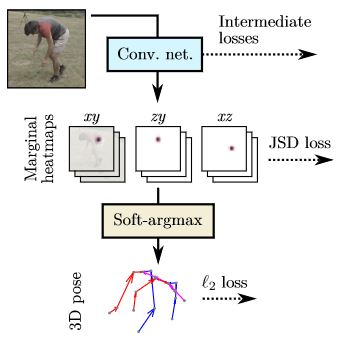
\includegraphics[height=7cm]{figures/nibali.JPG} 
        \caption{3D estimation from a single view~\cite{Nibali2019-yl}.}
        \label{subfig:single_view}
    \end{subfigure}
    \begin{subfigure}{0.49\textwidth}\centering
        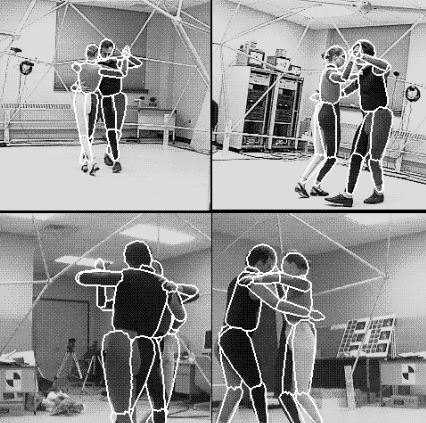
\includegraphics[height=7cm]{figures/gavrila.JPG}
        \caption{3D estimation from multiple views~\cite{gavrila19963}.}
        \label{subfig:multi_view}
    \end{subfigure}
    \caption{Examples of different approaches for 3D human pose estimation using RGB images from: (a) single and (b) multiple views.}
    \label{fig:3d_from_rgb}
\end{figure}

Another alternative for estimating three-dimensional locations from RGB images is combining multiple 2D views. Such is the case of the classic solution presented by Gavrila and Davis~\cite{gavrila19963}. They interpret the human body as a 3D graphical model with 22 degrees of freedom, in which each part is represented by superquadric geometric shapes. This model is fitted using frontal and lateral views of the subjects studied, as it is shown in Figure~\ref{subfig:multi_view}. More recently, Núñez \etal\cite{nunez2019multiview} proposed a pipeline that combines the usage of a \gls{cnn} and a \emph{Long-Short Term Memory Neural Network} for solving the same task. In their work, they estimate 2D coordinates in each view using the \gls{cnn} architecture proposed by Cao \etal in~\cite{cao2018openpose}. From these estimations, they minimize the reprojection error to 3D by using least-squares optimization. The final 3D estimations are refined taking advantage of temporal cues with the aforementioned \emph{Long-Short Term Memory Neural Network}.
 
 \subsection{From RGBD images}\label{subsec:from_rgbd_images}
The inclusion of depth measurements allows for higher accuracy in the estimated poses and better understanding of the scene being analyzed. It greatly reduces the ambiguity caused by the lost of information implicit in the 3D to 2D projection, even though it is still a challenging problem due to self-occlusions and limitations in image resolution. One of the most relevant approaches for human pose estimation from RGBD data is the one proposed by Shotton \etal\cite{shotton2011real}. In their work, they subdivide the estimation of the 3D coordinates in two tasks: per-pixel body parts recognition and joint coordinates inference. The former is solved as a multi-class pixelwise classification problem, modeled with a \emph{Randomized Decision Forest}. For the latter, they find modes in each labeled region using \emph{Mean Shift} clustering. An overview of this pipeline is shown in Figure~\ref{subfig:shotton}. This algorithm was introduced as a core component of the \emph{Kinect} gaming platform~\cite{han2013enhanced}. Another classic solution for this task is presented by Youding \etal\cite{Youding_Zhu2008-pr}. Using as input a video stream from a \emph{time-of-flight} sensor, they detect and track the position of anatomical landmarks using a probabilistic inference algorithm that optimizes a simple kinematic model. Schwarz \etal\cite{Schwarz2011-qi} try to solve the same task using geodesic distances and optical flow. A different approach is presented in~\cite{Ye2011-ui}, where Ye \etal estimate body pose by matching and refining pre-captured exemplars.

\begin{figure}[h]\centering
    \begin{subfigure}{0.55\textwidth}\centering
        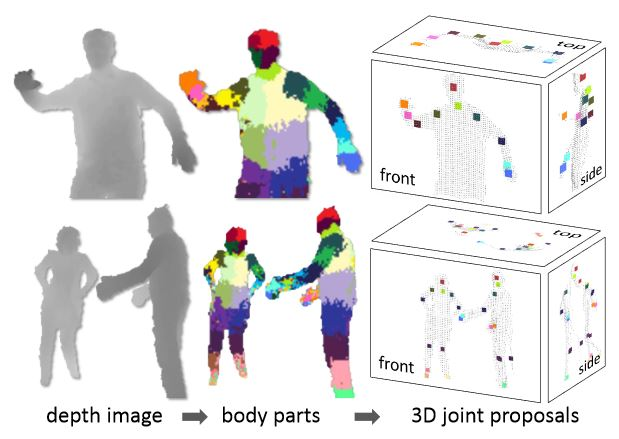
\includegraphics[height=6.25cm]{figures/shotton.JPG} 
        \caption{Shotton \etal proposal~\cite{shotton2011real}.}
        \label{subfig:shotton}
    \end{subfigure}
    \begin{subfigure}{0.44\textwidth}\centering
        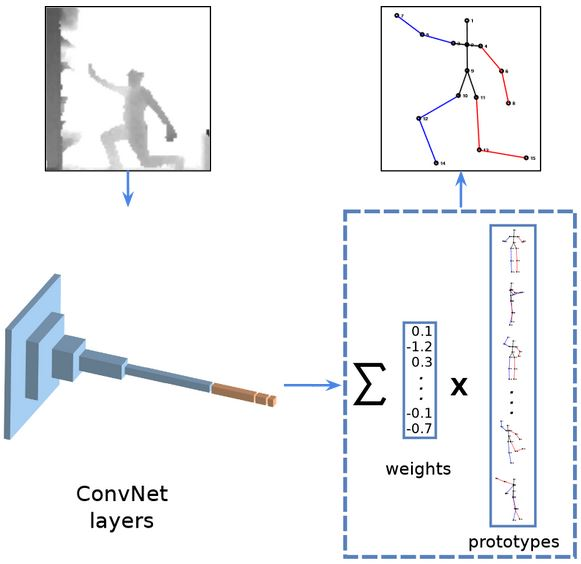
\includegraphics[height=6.25cm]{figures/marin_jimenez_adapted.JPG}
        \caption{Marín-Jiménez \etal approach~\cite{Marin-Jimenez2018-so}.}
        \label{subfig:marin}
    \end{subfigure}
    \caption{Examples of different approaches for 3D human pose estimation in RGBD images using (a) classic computer vision methods and (b) CNNs.}
    \label{fig:3d_from_rgbd}
\end{figure}

Recently, \gls{dl}-based solutions have been proposed to address pose estimation from depth maps. Marín-Jiménez \etal\cite{Marin-Jimenez2018-so} train a \gls{cnn} that estimates 3D body poses as a linear combination of prototype poses, as presented in Figure~\ref{subfig:marin}. Chang \etal\cite{Chang2018} introduce the novelty of designing their model as a 3D \gls{cnn}, which estimates the likelihood per voxel for each joint in the pose. They test their model performance not only for addressing human pose, but also hand pose estimation. In~\cite{Zimmermann2018-sn}, Zimmermann \etal use a 2D keypoint detector to estimate the 2D pose, which is next used together with the depth map as input to train a \gls{cnn} yielding predictions of real-world 3D coordinates. These 3D predictions are used for robotic tasks learning. This approach will be described in detail in Section~\ref{sec:3d_estimation_evaluation}, where we will compare the performance of our proposed pipeline against the results yielded by the Zimmermann \etal algorithm.